\section{有约束优化(二次规划问题)}
\subsection{问题}
利用有效集方法求解下述问题
\[
    \begin{aligned}
        \min & f(\boldsymbol{x}) = \dfrac{1}{2}\boldsymbol{x}^{\mathrm{T}}\boldsymbol{Hx} + \boldsymbol{c}^{\mathrm{T}}\boldsymbol{x}\\
        \operatorname*{s.t.} & \boldsymbol{A}_e\boldsymbol{x}-\boldsymbol{b}_e = \boldsymbol{0}\\
        & \boldsymbol{A}_i\boldsymbol{x}-\boldsymbol{b}_i \geqslant  \boldsymbol{0}
    \end{aligned}
\]
其中
\[
    \boldsymbol{H} = \begin{bmatrix}
        2 & -1\\
        -1 & 4
    \end{bmatrix},\quad\boldsymbol{c} = \begin{bmatrix}
        1 \\ 10
    \end{bmatrix}
\]
\[
    \boldsymbol{A}_e = [],\quad\boldsymbol{b}_e = []
\]
\[
    \boldsymbol{A}_i = \begin{bmatrix}
        -3 & -2\\
        1 & 0 \\
        0 & 1
    \end{bmatrix},\quad\boldsymbol{b}_i = \begin{bmatrix}
        -6 \\ 0 \\ 0
    \end{bmatrix}
\]

或者写为
\begin{equation}\label{eq:active_set}
    \begin{aligned}
        \min &\, f(\boldsymbol{x}) = x_1^2+2x_2^2-x_1x_2+x_1+10x_2\\
        \operatorname*{s.t.} &\, -3x_1-2x_2\geqslant -6\\
        &\, x_1\geqslant 0\\
        &\, x_2\geqslant 0
    \end{aligned}
\end{equation}
其约束的有效域为如图~\ref{fig:D-active_set}。
\begin{figure}[htbp]
    \centering
    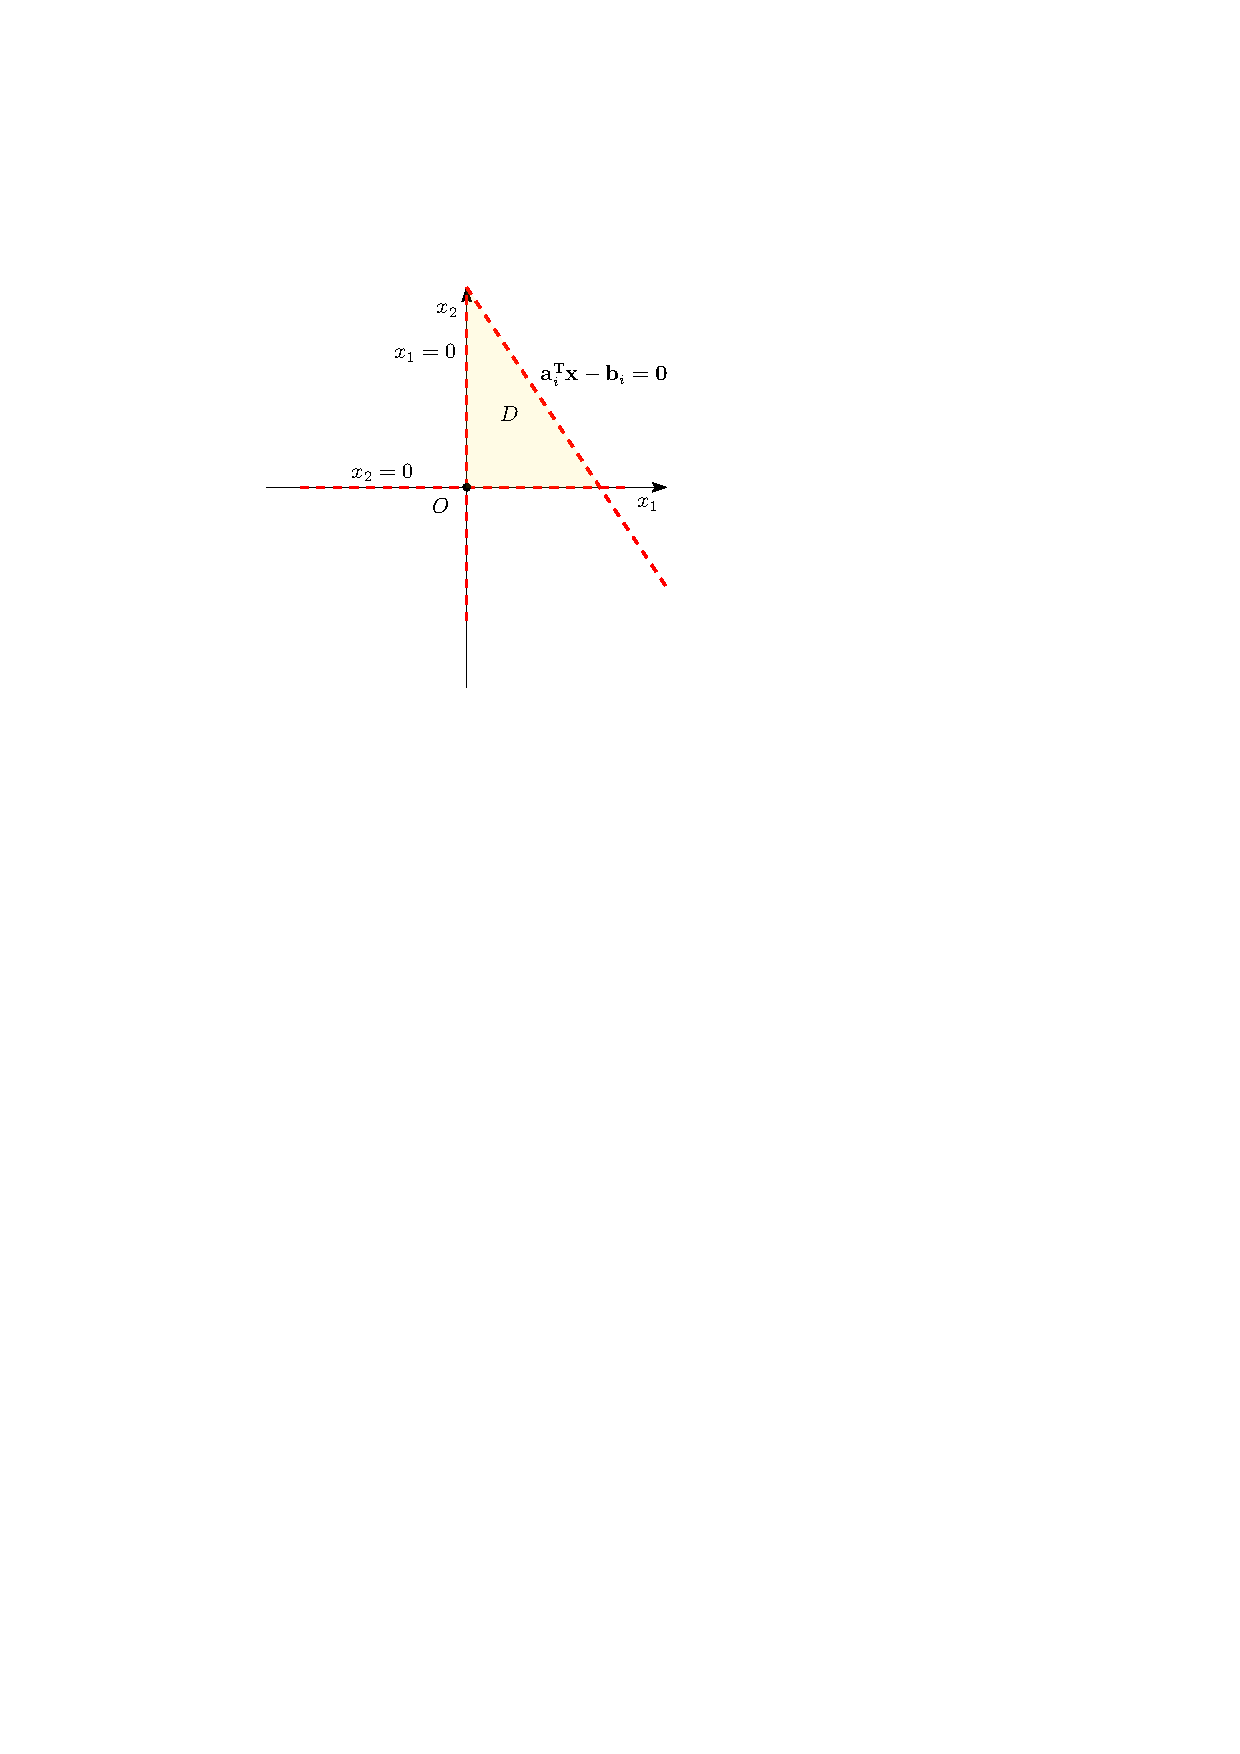
\includegraphics{image/active_set-image.pdf}
    \caption{问题~(\ref{eq:active_set})的有效域}
    \label{fig:D-active_set}
\end{figure}
\subsection{算法}
算法过程如图~\ref{fig:active_set-flow}。
\begin{figure}[H]
    \centering
    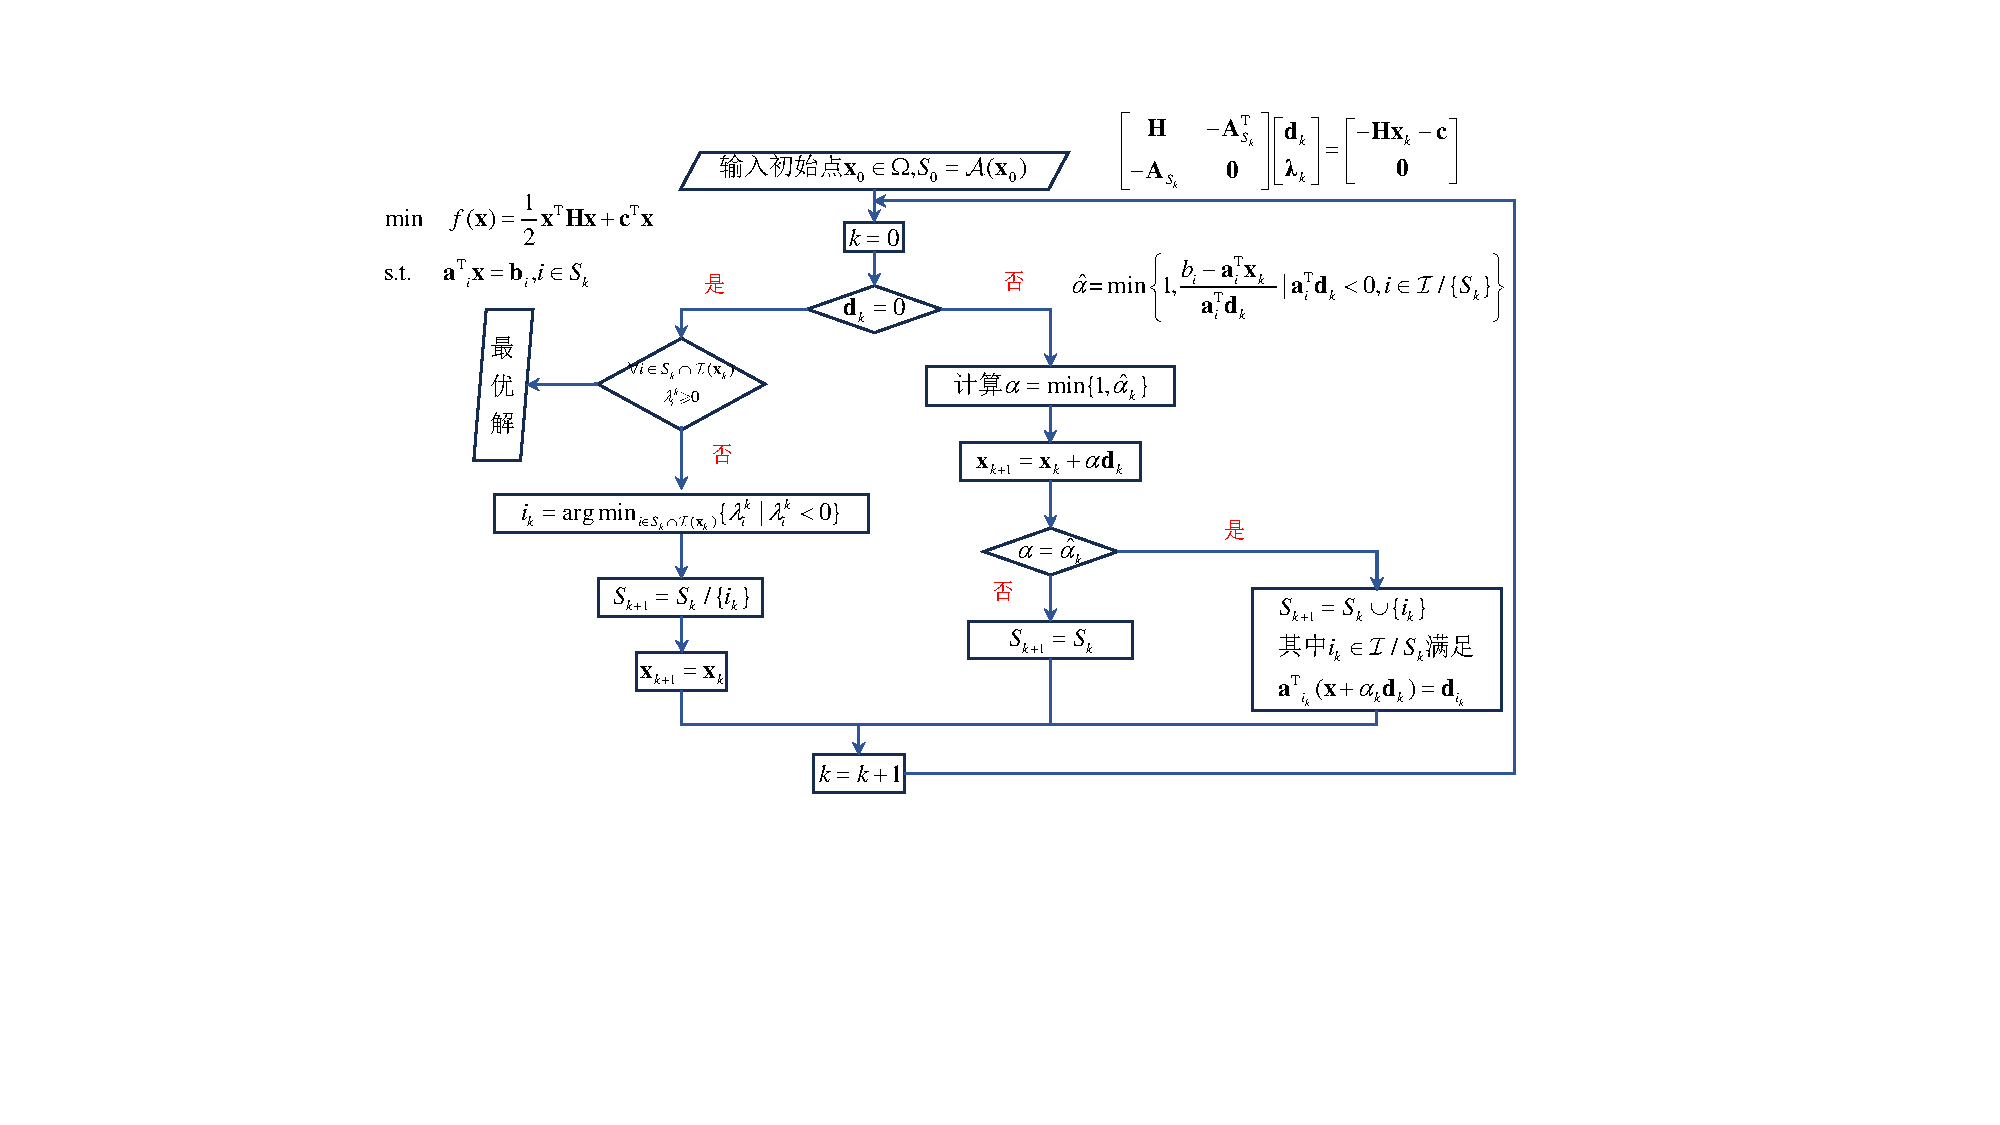
\includegraphics[width = .8\textwidth]{image/active_set-flow.pdf}
    \caption{有效集方法流程图}
    \label{fig:active_set-flow}
\end{figure}
\subsection{结果}
运行``active\_set.m''得到迭代序列如图~\ref{fig:active_set-matlab}。
\begin{figure}[H]
    \centering
    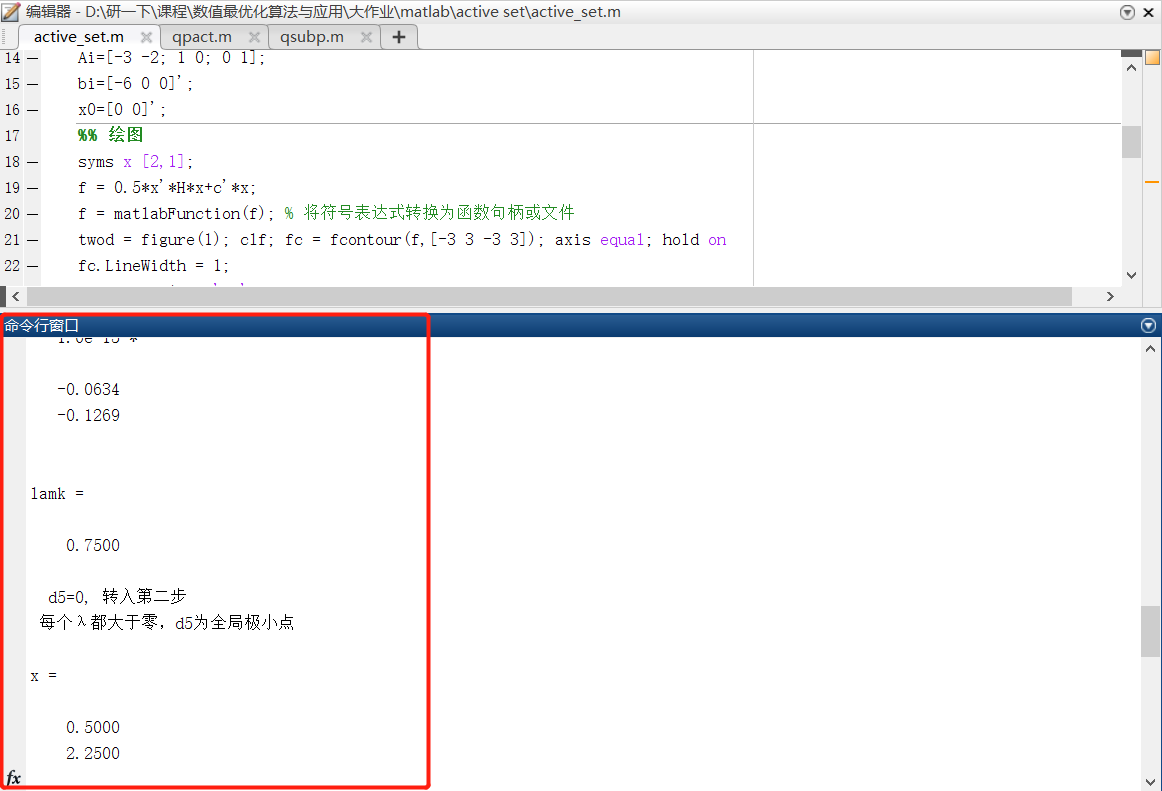
\includegraphics[width = .8\textwidth]{image/active_set-matlab.png}
    \caption{运行`active\_set.m'得到迭代序列}
    \label{fig:active_set-matlab}
\end{figure}

算法得到的数值最优解$\boldsymbol{x}^*$
\[
    \boldsymbol{x}^* = \left( 0.5000,2.2500 \right)^{\mathrm{T}}
\]


算法迭代过程如图~\ref{fig:Active_set}。
\begin{figure}[htbp]
    \centering%
    \subfloat[基于有效集方法的梯度下降法2d迭代]{%
        \label{fig:Active_set-2d}
        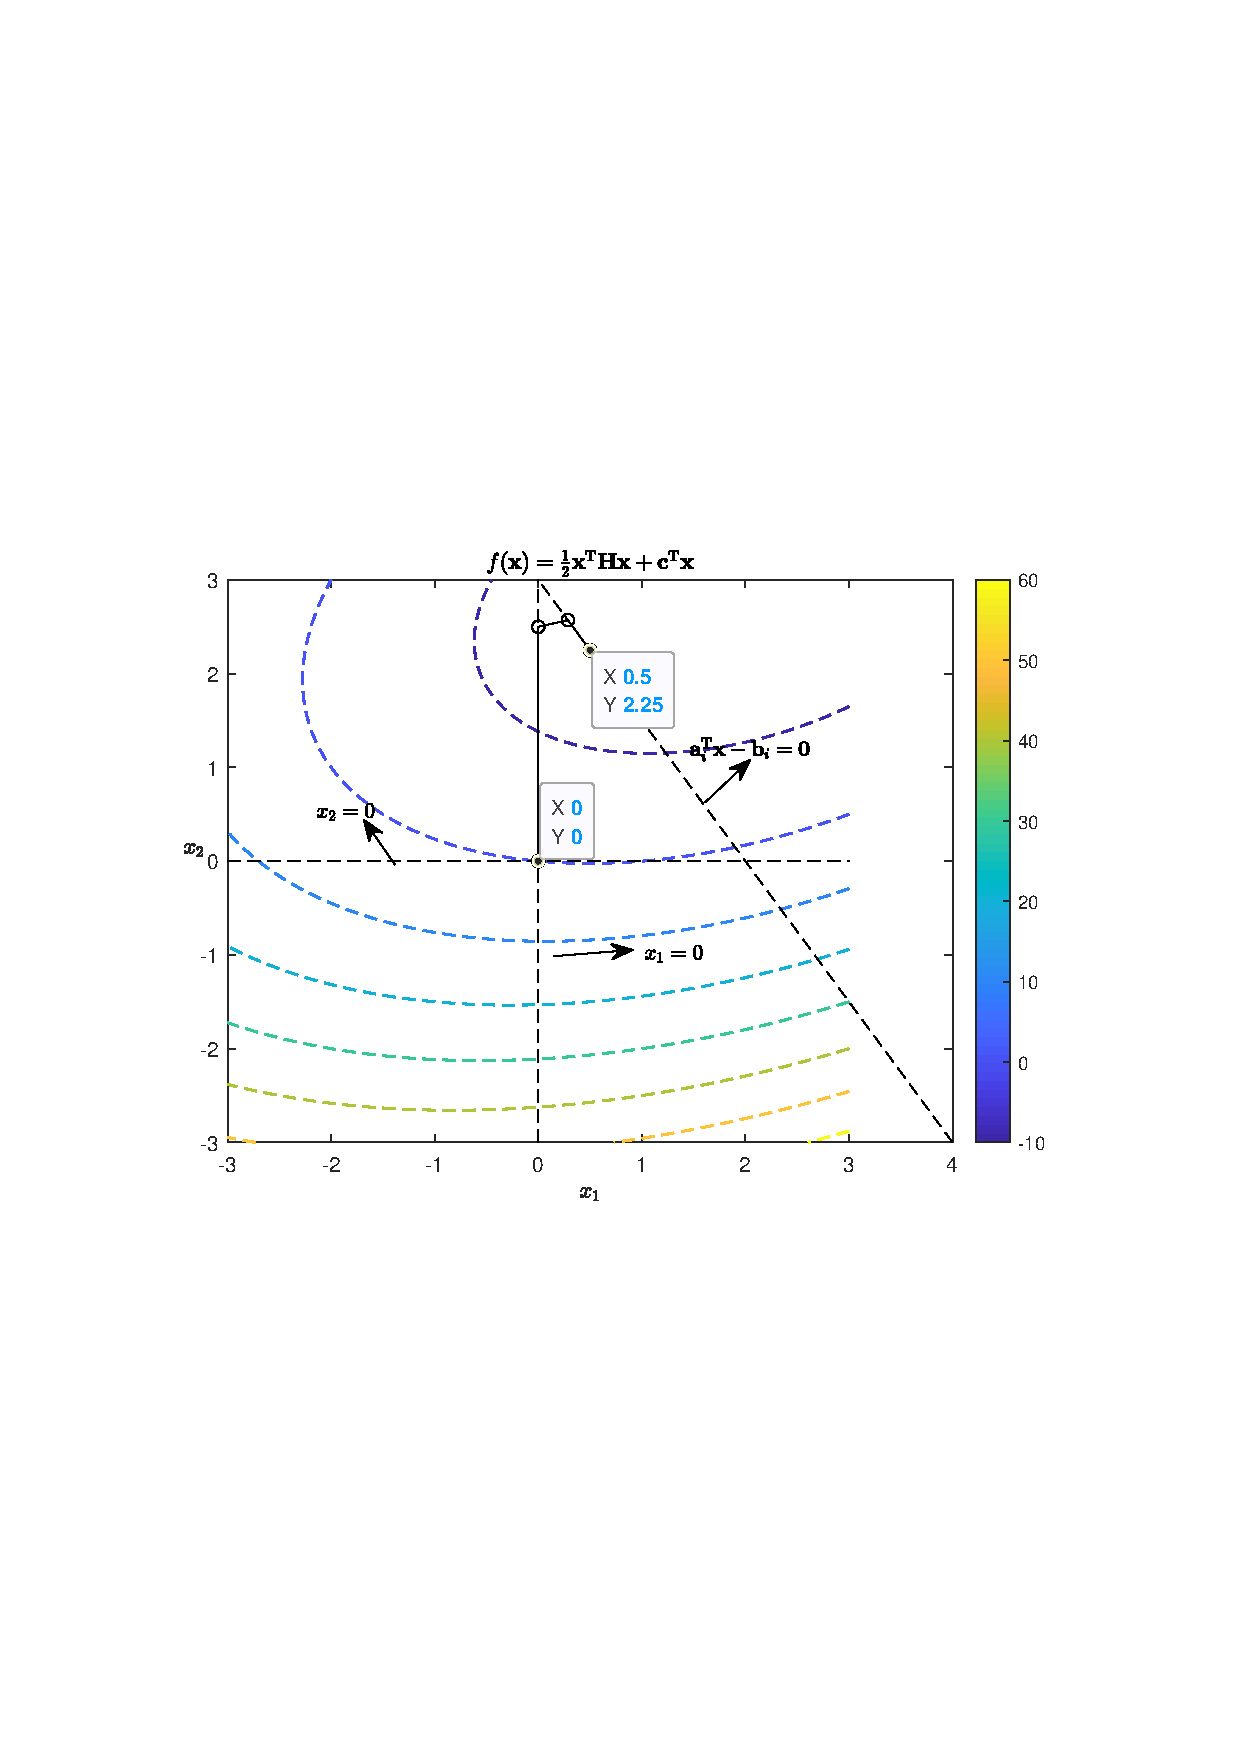
\includegraphics[width = .45\textwidth]{image/active_set-2d.pdf}}\hspace{.5em}%
    \subfloat[基于有效集方法的梯度下降法3d迭代]{%
      \label{fig:Active_set-3d}
      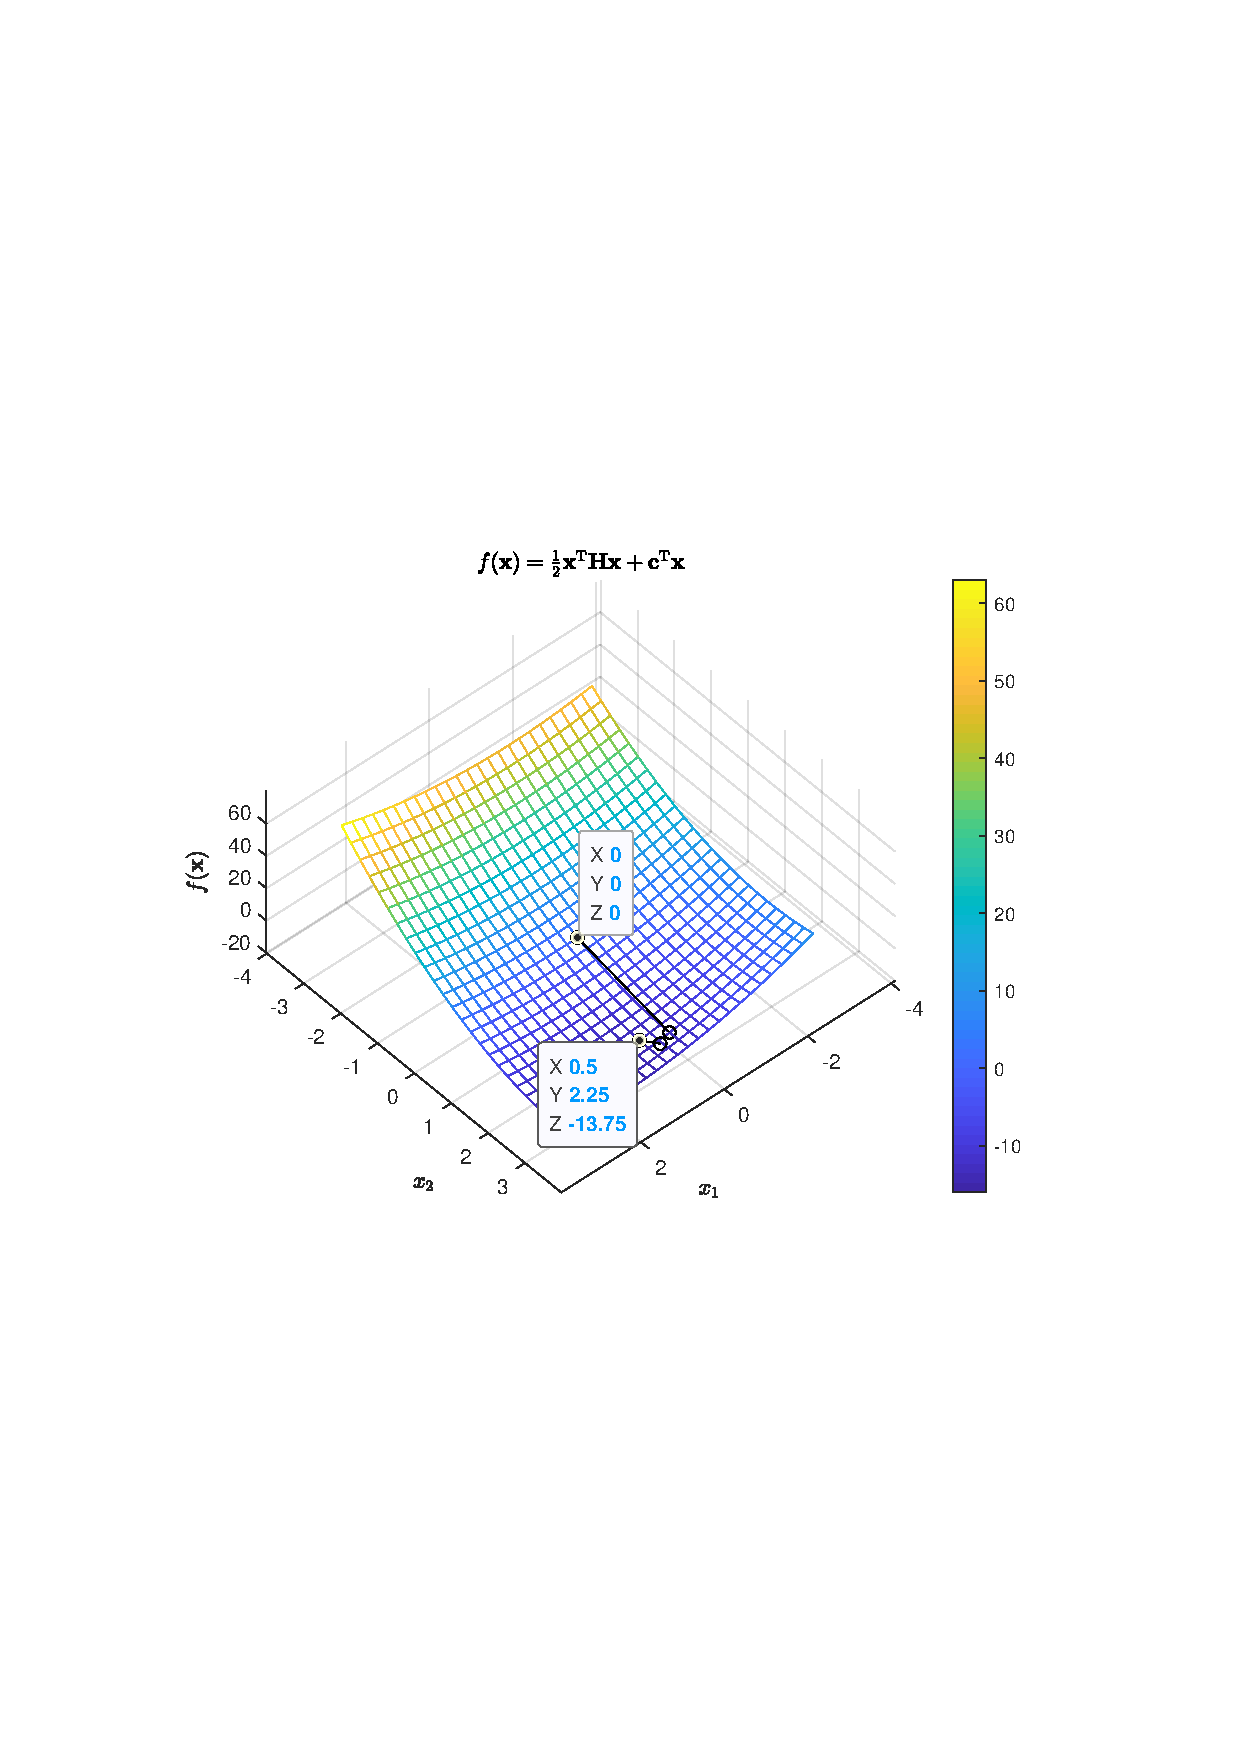
\includegraphics[width = .45\textwidth]{image/active_set-3d.pdf}}
    \caption{有效集方法}
    \label{fig:Active_set}
\end{figure}
% \[
%     \begin{bmatrix}
%         \boldsymbol{H} & -\boldsymbol{A}_{S_{k}}^{\mathrm{T}} \\
%         -\boldsymbol{A}_{S_{k}} & \boldsymbol{0}
%     \end{bmatrix}
%     \begin{bmatrix}
%         \boldsymbol{d}_{k}\\\boldsymbol{\lambda}_{k}
%     \end{bmatrix}=
%     \begin{bmatrix}
%         -\boldsymbol{Hx}_{k}-\boldsymbol{c}\\
%         \boldsymbol{0}
%     \end{bmatrix}
% \]
\subsection{代码}
有效集方法求解、子问题求解和主函数分别见代码~\ref{code:qpact}、\ref{code:qsubp}和~\ref{code:active_set}。
\lstinputlisting[
    language    =   matlab,
    style       =   elegantcode,
    caption     =   {有效集方法代码},
    label       =   {code:qpact}
]{code/qpact.m}
\lstinputlisting[
    language    =   matlab,
    style       =   elegantcode,
    caption     =   {子问题代码},
    label       =   {code:qsubp}
]{code/qsubp.m}
\lstinputlisting[
    language    =   matlab,
    style       =   elegantcode,
    caption     =   {主函数代码},
    label       =   {code:active_set}
]{code/active_set.m}